\documentclass{beamer}


\graphicspath{{figures/}}
\usepackage{tikz}
\usetikzlibrary{positioning, arrows}
%\usetheme{boxes}
\usepackage[utf8]{inputenc}
\usepackage{amsmath}
\usepackage{amsthm}
\usepackage{hyperref}
\usepackage[font=tiny]{caption}
\usepackage{booktabs}
\usepackage{natbib}
\bibliographystyle{plainnat}
\usecolortheme{crane}

\definecolor{orange}{RGB}{232, 86, 15}
\definecolor{blue}{RGB}{14, 159, 232}
\definecolor{blueblue}{RGB}{50, 90, 160}
\definecolor{yellow}{RGB}{232, 187, 14} 
\definecolor{red}{RGB}{232, 14, 59}

\hypersetup{
  colorlinks=true,
  linkcolor=cyan,
  urlcolor=cyan,
  citecolor=purple
}
\newtheorem{deff}{Definición}
%Information to be included in the title page:
\institute[]{}

\setbeamercolor{title}{bg=blueblue, fg=white}
\setbeamercolor{subttile}{bg=blueblue, fg=white}
\setbeamercolor{frametitle}{bg=blueblue, fg=white}
\setbeamercolor{block title}{bg=blue, fg=white}
\setbeamercolor{block title alerted}{bg=red, fg=white}
\setbeamercolor{block title example}{bg=yellow, fg=white}
\setbeamercolor{footline}{bg=gray, fg=white}

\beamertemplatenavigationsymbolsempty

\newcommand{\indep}{\perp \!\!\! \perp}
\title{(Casual) Causality Course 2025 \\ Session 2}
\author{Gherardo Varando}
\date{27 March 2025}
\begin{document}

\begin{frame}
\maketitle
\end{frame}

\begin{frame}{(Casual) Causality Course 2025}

	\begin{block}{Intructors}
	  \begin{itemize}
	    \item Gherardo \url{gherardo.varando@uv.es}
	    \item Emiliano \url{emiliano.diaz@uv.es} 
	    \item Vassilis \url{vasileios.sitokonstantinou@uv.es}
	  \end{itemize}
	\end{block}
	
	\begin{block}{Schedule} 
         \begin{itemize}
	   \item \textbf{week 1, Tuesday} Intro and causal inference (GV)
	   \item \textbf{week 1, Thursday} Causal inference and robustness (GV)    
	   \item \textbf{week 2, Tuesday} Causal Discovery (ED)
	   \item \textbf{week 2, Thursday} Causal Discovery (ED)
	   \item \textbf{week 3} Intensive weeek with group projects! 
	 \end{itemize}
	\end{block}


\end{frame}


\begin{frame}{Content week 1}
  \begin{itemize}
    \item \textbf{Session 1} Tue 25/03
      \begin{itemize}
	\item[Part I] \textbf{Intro to causality and causal methods} \\ 
	  \only<2>{motivation, causal questions, what is causality? \\
		      experiments, interventions and counterfactuals \\ 
		      structural causal models and graphs}
         \item[Part II] \textbf{Basics of causal inference} \\
	     \only<2>{causal effect, randomized experiments  \\
	              observational studies, identifiability conditions \\
		      graphical representation, confounding, selection bias \\
		      random variability and measurement error 
	   } 
      \end{itemize}
\vfill
    \item \textbf{Session 2} Thu 27/03
      \begin{itemize}
	\item  Causal inference methods
      \end{itemize}
  \end{itemize}
\end{frame}

\begin{frame}{Basic references}
  \begin{itemize}
    \item \href{https://mitpress.mit.edu/9780262037310/elements-of-causal-inference/}{Elements of causal inference} \citep{peters2017elements} [EC] 
    \item \href{https://miguelhernan.org/whatifbook}{Causal Inference: What If} \citep{hernan2025causal} [Wif]
    \item All of Statistics \citep{wasserman2013all} [AoS] 
  \end{itemize}

  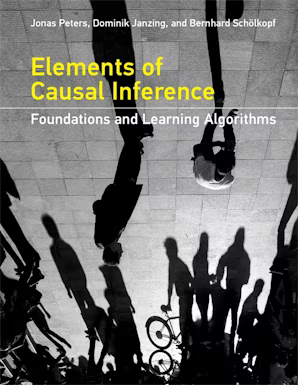
\includegraphics[width = 2 cm]{elements}
  
\includegraphics[width = 2 cm]{whatif}
  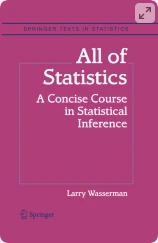
\includegraphics[width = 2 cm]{all}
\end{frame}


\begin{frame}{What is causality?}
  \begin{columns}
    \begin{column}{0.7\textwidth}
  %\begin{center}
  %  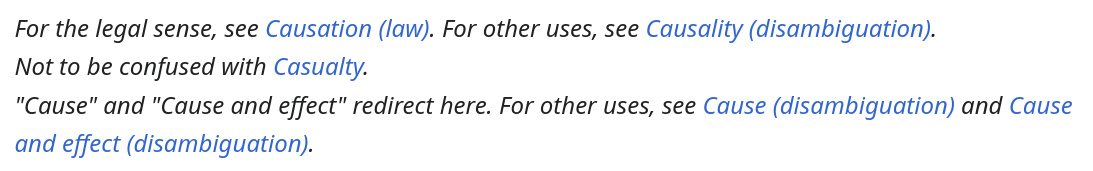
\includegraphics[width=0.95\textwidth]{Causality-Wikipedia}
  %\end{center}
  \begin{itemize}
    \item Causality in Law  \url{https://en.wikipedia.org/wiki/Causation_(law)} \\
      \href{https://www.youtube.com/watch?v=XiCOmhdkM80&list=PLqMxKp2ot-3vDaLyaAZNgt8ijj6n0l460}{Causation|Low of Tort playlist on youtube, first 3 videos}  
    \item Rethinking Actual Causation in Tort Law \url{https://harvardlawreview.org/print/vol-130/rethinking-actual-causation-in-tort-law/}
    \item Causality in Physics \\
       \url{https://en.wikipedia.org/wiki/Causality_(physics)}  \\
       \url{https://www.youtube.com/watch?v=eG_eHDDMgCs} \\
       \cite{rovelli2022causationrootedthermodynamics}  
  \end{itemize}
  \end{column}
    \begin{column}{0.3\textwidth}
       \begin{figure}
	 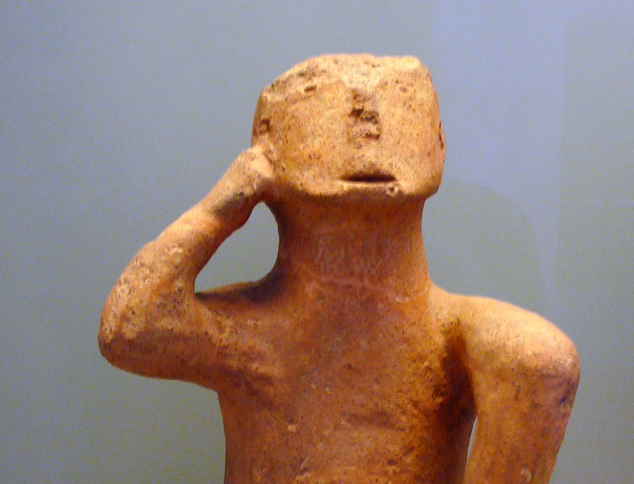
\includegraphics[width=3cm]{thinker1}
	 \caption{Karditsa Thinker at the National Archaeological Museum, Athens} 
       \end{figure}
       \vfill
    \onslide<2->{
      \begin{itemize}
	  \tiny
	\item Work in groups and briefly discuss causality in physics or law 
	      \textbf{[15 min]}, choose a speaker 
	    \item  The two speakers present the main ideas \textbf{[5 min]} (whiteboard, slides)
      \end{itemize}
    }
    \end{column}
  \end{columns}
\end{frame}


\begin{frame}{Potential outcomes - Counterfactual model}
  \begin{columns}
    \begin{column}{0.5\textwidth}
  \cite{hernan2025causal} \cite{wasserman2013all}  
  \begin{itemize}
    \item consider a binary \textbf{treatment variable} $A$
      (1: forest management practice (thinning, controlled burns,...) , 0: wild/uncontrolled forest)
    \item and a binary \textbf{outcome} $Y$ (1: burned area, 0: not burned)
    \item $A,Y$ are random variables that take possible different values for each individual
  \end{itemize}
  \vfill
    \end{column}
    \begin{column}{0.5\textwidth}
      \begin{figure}
      \includegraphics[width = \textwidth]{burn}
	\caption{From \url{https://www.kunc.org/2024-03-15/long-term-study-finds-combination-of-prescribed-burns-thinning-effective-at-reducing-wildfire-risk}} 
      \end{figure}
    \end{column}
  \end{columns}

\end{frame}


\begin{frame}{Potential outcomes - Counterfactual model}
  \begin{columns}
    \begin{column}{0.5\textwidth}
  \cite{hernan2025causal} \cite{wasserman2013all}  
  \begin{itemize}
    \item<1-> denote with the outcome variable that would have been observed under treatment $a=1$, and similarly $Y^{a=0}$
    \item<2-> $Y^{a=1}$ and $Y^{a=0}$ are called \textbf{potential outcomes} or \textbf{counterfactual outcomes}
    \item<3-> for each individual, only one of the potential outcomes
      is actually observed/factual.
      \[ Y = Y^{a=A}  \quad \text{(consistency equation)} \]
  \end{itemize}
    \end{column}
    \begin{column}{0.5\textwidth}
      \begin{figure}
      \includegraphics[width = \textwidth]{burn}
	\caption{From \url{https://www.kunc.org/2024-03-15/long-term-study-finds-combination-of-prescribed-burns-thinning-effective-at-reducing-wildfire-risk}} 
      \end{figure}
    \end{column}
  \end{columns}

\end{frame}


\begin{frame}{Causal effects}
  \begin{definition}{Average causal effects}
    An average causal effect of treatment $A$ on outcome $Y$ is present if
    \[ P(Y^{a=1} = 1) \neq   P(Y^{a=0} = 1) \]
    or equivalently (for binary outcomes)
    \[ \mathbb{E}[Y^{a=1}] \neq \mathbb{E}[Y^{a=0}] \]
  \end{definition}
  \begin{itemize}
    \item<2-> in practice we need to \textbf{measure} causal effects
    \item<3-> {causal risk difference} $P(Y^{a=1} = 1) - P(Y^{a=0} = 1)$
    \item<4-> {causal risk ratio} $\frac{P(Y^{a=1} = 1)}{P(Y^{a=0} = 1)}$
    \item<5-> {causal odds ratio} $\frac{P(Y^{a=1} = 1) / P(Y^{a=1} = 0) }{P(Y^{a=0} = 1) / P(Y^{a=0} = 0)}$
  \end{itemize}
\end{frame}



\begin{frame}{Randomized experiments}
  \begin{columns}

    \begin{column}{0.5\textwidth}
  \begin{itemize}
    \item<1-> We collect data following a randomized control study:
      for each individual (forest unit/patch)  we flip a coin and we assign the treatment variable
      to be $a=1$ if heads and $a=0$ if tails.
    \item<2-> We then collect the outcome variable $Y$ (e.g. burned or not after 1 year) for all individuals in
      the study
  \end{itemize}
    \end{column}
    \begin{column}{0.5\textwidth}
     \begin{figure}
       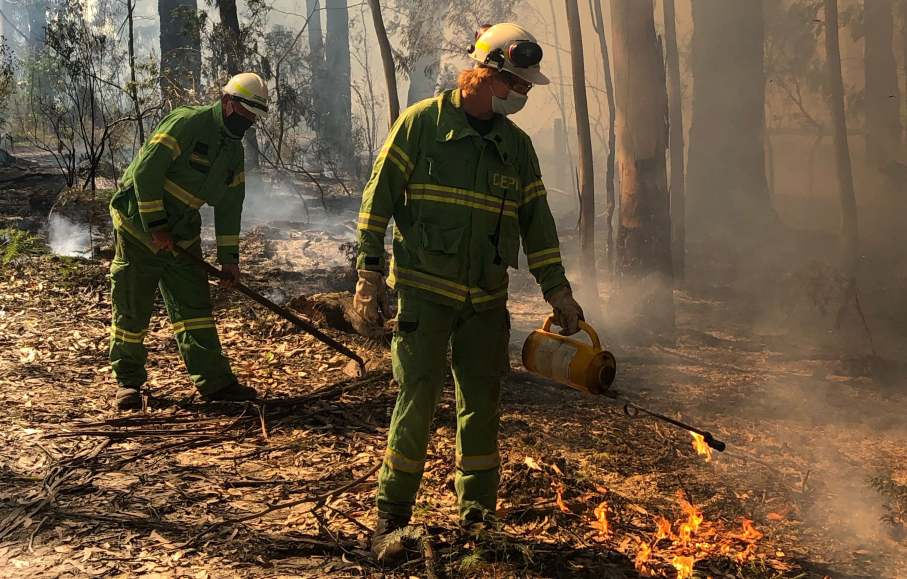
\includegraphics[width = \textwidth]{crew}
     \end{figure}
    \end{column}
  \end{columns}
\end{frame}

\begin{frame}{Randomized experiments}
  \begin{columns}

    \begin{column}{0.5\textwidth}
  \begin{itemize}
    \item<1-> assume no problem with the study, everybody is following instruction and
      there are no measurements problems (\emph{ideal randomized experiment})
    \item<2-> can we say something about the causal effect of $A$ on $Y$ ?
    \item<3-> yes! we can compute the average causal effect ... formally because there
      is \textbf{exchangeability} between the treated ($A=1$) and untreated ($A=0$) groups
  \end{itemize}
    \end{column}
    \begin{column}{0.5\textwidth}
     \begin{figure}
       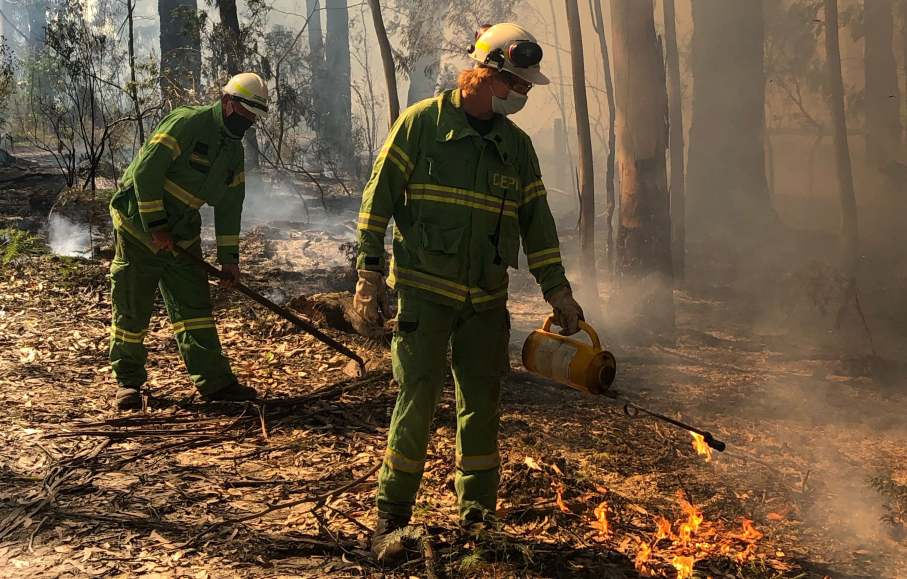
\includegraphics[width = \textwidth]{crew}
     \end{figure}
    \end{column}
  \end{columns}
\end{frame}

\begin{frame}
	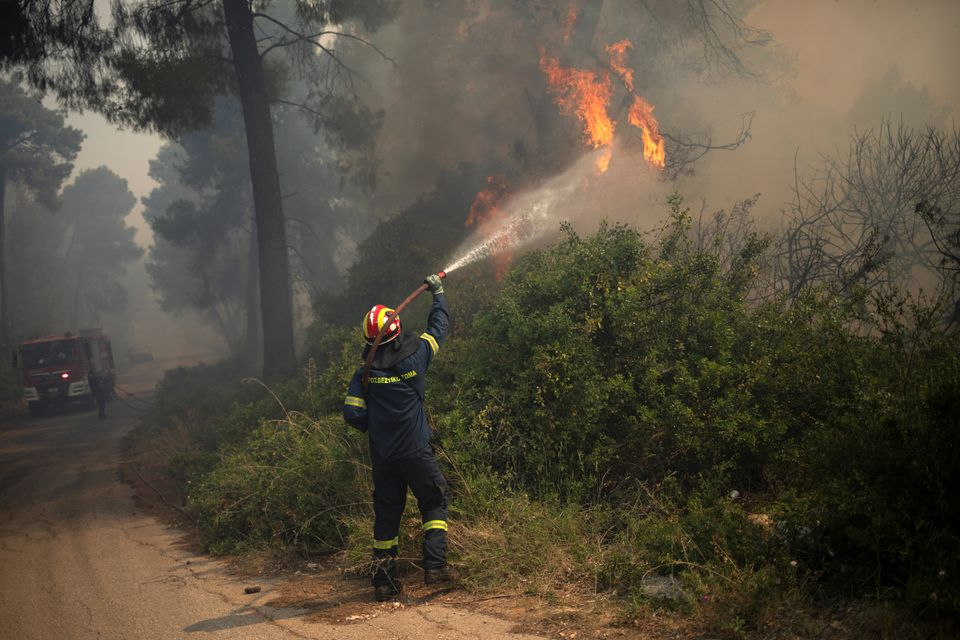
\includegraphics[scale=0.2]{fire}

	\textbf{New problem: the firefighters do not like your randomized study}
	they say that it is too dangerous not to manage some patches at all, and that some
	areas have a too high fire risk to be left completely untreated
\end{frame}

\begin{frame}{Conditional randomized experiments}
  \begin{itemize}
    \item<1-> Assume we have now a covariate $L$, measured before treatment was assigned
      (e.g. risk of fire: low, medium, high)
    \item<2-> We divide the population into strata based on the levels of $L$
      and we perform randomization with different probabilities in each stratum
    \item<3-> In each stratum, we have exchangeability and we can compute
      average treatment effects
    \item<4-> this is called \emph{stratification}
    \item<5-> moreover we say that this procedure ensure \textbf{conditional exchangeability}                          $Y^a \indep A | L$
  \end{itemize}
\end{frame}

\begin{frame}{Computing ATE from conditionally randomized data}
	\begin{itemize}
		\item<1-> From the data collected with a conditionally randomized experiment we can compute
			the ATE in all population.
		\item<2-> \textbf{Standardization} consists in computing the
			marginal counterfactual risk
			as the weighted average of the stratum-specific risk.
			\[ P(Y^a = 1) = \sum P(Y^a = 1| L = l)P(L = l) \]
		\item<3-> \textbf{Inverse Probability Weighting} is an alternative, but equivalent,
			procedure to compute $P(Y^a = 1)$ by weighting each individual sample
			by $w_l = 1 / P(A = a|L = l)$ and then we compute $P(Y^a = 1) = \sum w_l P(Y | A= a, L = l)$
	\end{itemize}
\end{frame}



\begin{frame}{Observational studies}
	Sometimes is unethical, too expensive or simply impossible to conduct experiments, so we are left only with observational data, what can we do? (e.g. we just collect historical
	data on forest management practice  and burned areas)
	\begin{itemize}
		\item<2-> Problems: confounding variables (e.g. forest are controlled more when we expect to
			have high risk of fire, patients are treated with more invasive/effective treatments when doctors thinks the case is more serious, \ldots)
		\item<3->  still under certain conditions and assumptions we can identify the
			causal effect
		\item<4-> this conditions 
		  \emph{assure that the observational study can be used
			somehow as a randomized trial}
	\end{itemize}
\end{frame}

\begin{frame}{Identifiability conditions}
  \begin{enumerate}
    \item<1-> \textbf{Exchangeability} the conditional probability
      of receiving every value of treatment, though
      not decided by the investigators, depends only on measured covariates $L$
    \item<2-> \textbf{Positivity} the probability of
      receiving every value of treatment conditional on $L$ is
      greater than zero, i.e., positive
    \item<3-> \textbf{Consistency} the values of treatment under comparison
      correspond to well-defined interventions that,
      in turn, correspond to the versions of treatment in the data
  \end{enumerate}
  \only<4>{If we can assume this three conditions we can use the techniques such as IPW or standardization to compute ATE from observational data}
\end{frame}

\begin{frame}{Effect modification}

  \begin{itemize}
    \item We say that $V$ is a modifier of the effect of $A$ on $Y$
      when the average causal effect of $A$ on $Y$ varies across levels of $V$
    \item \textbf{Stratification} or \textbf{matching} can be used to identify effect modification
    \item<2-> To construct our matched population we replaced the treated in the 
      population by a subset of the treated in which the matching factor $L$ had the
      same distribution as that in the untreated.
    \item<3-> they require exchangeability and positivity
    \item<4-> Standardization (or IPW), stratification and matching measure different
      causal effects: Average effects in the entire population, conditional causal effects (startification) and usually causal effects in the treated and untreated for matching
  \end{itemize}

\end{frame}

\begin{frame}{Computing interventional distributions in SCM}
  \begin{block}{\small truncated factorization~\citep{pearl1993belief},
    G-computation formula~\citep{robins1986new},
    manipulation theorem~\citep{spirtes2000causation}}
    Given an SCM $\mathcal{C}$ and an intervened SCM $\tilde{\mathcal{C}}$, obtained
    from $\mathcal{C}$ by intervening on some $X_k$ with $k \neq j$, we have that
    \[P^{\tilde{\mathcal{C}}}(X_j |  X_{pa(j)}) = P^{\mathcal{C}}(X_j | X_{pa(j)})\]

  \end{block}
  \begin{itemize}
    \item<1-> Combining the above property and the assumption of SCM we can sometimes
      compute interventional distribution from observational quantities
    \item<2-> Thus in practical terms we will be able sometimes to
      estimate interventional objects, such as treatment effects, from
      observational data alone
    \item<3-> This requires the \emph{knowledge of the causal graph}
  \end{itemize}

\end{frame}

\begin{frame}{Confounding and adjusting}
  \begin{itemize}
    \item<1-> Consider an SCM $\mathcal{C}$, the causal effect from $X$ to $Y$ is called confounded if $P^{\mathcal{C}, do(X = x)}(y) \neq P^{\mathcal{C}}(y)$ 
    \item<2-> $\mathbf{Z}$ is called a valid adjustment set for $X,Y$ if 
      \[ P^{\mathcal{C}, do(X = x)}(y) = \sum P^{\mathcal{C}}(Y| X, \mathbf{Z} = z)P^{\mathcal{C}}(\mathbf{Z}=\mathbf{z}) \]
    \item<3-> Valid asjustment sets are: 
      \begin{enumerate}
	\item \textbf{parent adjustment} $PA_X$ 
	\item \textbf{backdoor criterion} Any $\mathbf{Z}$ such that i) contains no descendant of X and ii) blocks all backdoor paths $\rightarrow X$ 
	\item \textbf{towards necessity}  \ldots 
      \end{enumerate}
    \item<4-> Valid adjustment sets ensure conditional exchangeability, thus we can use standardization or stratification to compute average or conditional causal effect 
    \item<5-> viceversa there are techniques that can handle confounding problems without relying on exchangeability: e.g. difference-in-differences, instrumental variables and 
      the front door criterion
  \end{itemize}
\end{frame}

\begin{frame}{Selection bias} 
  \begin{center}
    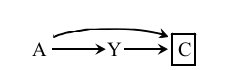
\includegraphics[scale=1]{selection}
  \end{center}
  \begin{itemize}
    \item<1-> If we condition on $C$ there are two open paths between $A$ and $Y$ 
    \item<2-> This can happen for example: differential loss to follow-up, missing data bias, nonresponse bias, healthy worker bias, self-selection bias, volunteer bias, 
      and selection affected by treatment received before study entry 
    \item<3-> Selection bias leads to a lack of exchangeability
    \item<4-> IPW or stratification can be used to control for selection bias 
    \item<5-> randomization does not protect from selection bias 
  \end{itemize}
\end{frame}


\begin{frame}{Do-calculus}
  \begin{itemize}
    \item<1-> an interventional distribtuion in an SCM is called identifiable if it can be computed from observational quantities and properties of the graph structure 
    \item<2-> Pearl has developed the so-called \textbf{do-calculus} that consists in a set of three rules: Insertion/deletion of observations, Action/observation exchange, Insertion/deletion of actions
    \item<3-> do-caluclus is complete, every identifiable interventional distribution can be obtained 
    \item<4-> one corollary of the do-calculus theorem is the \textbf{front-door adjustment} 
  \end{itemize}

\end{frame}

\begin{frame}
	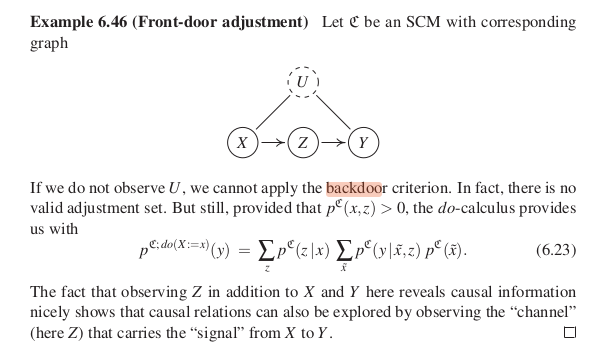
\includegraphics[scale=0.5]{front}
\end{frame}

\begin{frame}[allowframebreaks]{Bibliography}
  \tiny
\bibliography{biblio}
\end{frame}

\end{document}


